% Figure 10 of "Galashin's Conjecture 4.3 via a convex gradient": every crossing column of M_N as a half-open arc of necklace rows.
% Source of the figure, typeset in the paper's own fonts (T1, Latin Modern, 11pt) at the paper's text
% width (6.5in), so \includegraphics does not rescale it. Illustrates CLH-4; it adds no assertion.
% Every value drawn is read from these Lean output lines:
%   S2EX02 window(1-based)=[3, 5, 1, 2, 4] n=5 columns=7
%   S2EX02 s_x (x=1..n)=[3, 4, 1, 5, 2]
%   S2EX02 edgeOf j (j=1..columns, paper labels)=[(1, 2), (2, 3), (2, 4), (3, 5), (4, 5), (5, 1), (5, 2)]
%   EX02 M=[[0, -1, 0, 0, -1, 0, 0], [0, 0, 0, -1, -1, 0, 0], [0, 0, 0, 0, 0, -1, -1], [-1, 0, 0, 0, 0, 0, -1], [0, -1, -1, 0, 0, 0, 0]]
%   S2EX02 arc rows (s_t,s_h] per column j (rows 1-based)=[[4], [1, 5], [5], [2], [1, 2], [3], [3, 4]]
% Build: pdflatex <this file> && pdftocairo -svg <this file>.pdf <this file>.svg
\documentclass[11pt]{standalone}
\usepackage[T1]{fontenc}
\usepackage{lmodern}
\usepackage{amsmath,amssymb}
\usepackage{tikz}
\usetikzlibrary{arrows.meta,positioning,calc}

% the palette of the paper's other figures: blue solid for the first strand or arc, ochre dashed for the second
\definecolor{ink}{HTML}{233740}
\definecolor{muted}{HTML}{65757D}
\definecolor{pblue}{HTML}{0072B2}
\definecolor{qochre}{HTML}{B87827}

\tikzset{
  base/.style={draw=muted, line width=0.5pt},
  exit/.style={circle, draw=ink, fill=white, line width=0.6pt, inner sep=0pt, minimum size=4.6pt},
  entry/.style={circle, draw=ink, fill=ink, line width=0.6pt, inner sep=0pt, minimum size=4.6pt},
  exitP/.style={exit, draw=pblue}, entryP/.style={entry, draw=pblue, fill=pblue},
  exitQ/.style={exit, draw=qochre}, entryQ/.style={entry, draw=qochre, fill=qochre},
  strandP/.style={pblue, line width=1.1pt, -{Stealth[length=5pt,width=4.2pt]}, shorten >=2.4pt},
  strandQ/.style={qochre, line width=1.1pt, dash pattern=on 4pt off 1.6pt, -{Stealth[length=5pt,width=4.2pt]}, shorten >=2.4pt},
  lab/.style={font=\footnotesize, inner sep=1.2pt, text=ink},
  labm/.style={font=\small, inner sep=1.2pt, text=ink},
  labP/.style={font=\small, inner sep=1.2pt, text=pblue},
  labQ/.style={font=\small, inner sep=1.2pt, text=qochre},
  muted text/.style={text=muted},
  ttl/.style={font=\small, text=ink, inner sep=0pt},
  negE/.style={font=\small, text=pblue, inner sep=0pt},
  posE/.style={font=\small, text=qochre, inner sep=0pt},
  zeroE/.style={font=\small, text=ink, inner sep=0pt},
  idx/.style={font=\footnotesize, text=muted, inner sep=0pt},
}
\tikzset{
  cellin/.style={circle, draw=pblue, fill=pblue!9, line width=0.8pt, double=pblue!9, double distance=1.1pt, inner sep=0pt, minimum size=0.62cm, font=\small, text=pblue},
  cellout/.style={circle, draw=muted!45, dash pattern=on 1.6pt off 1.4pt, line width=0.6pt, inner sep=0pt, minimum size=0.62cm, font=\small, text=muted},
}

\begin{document}
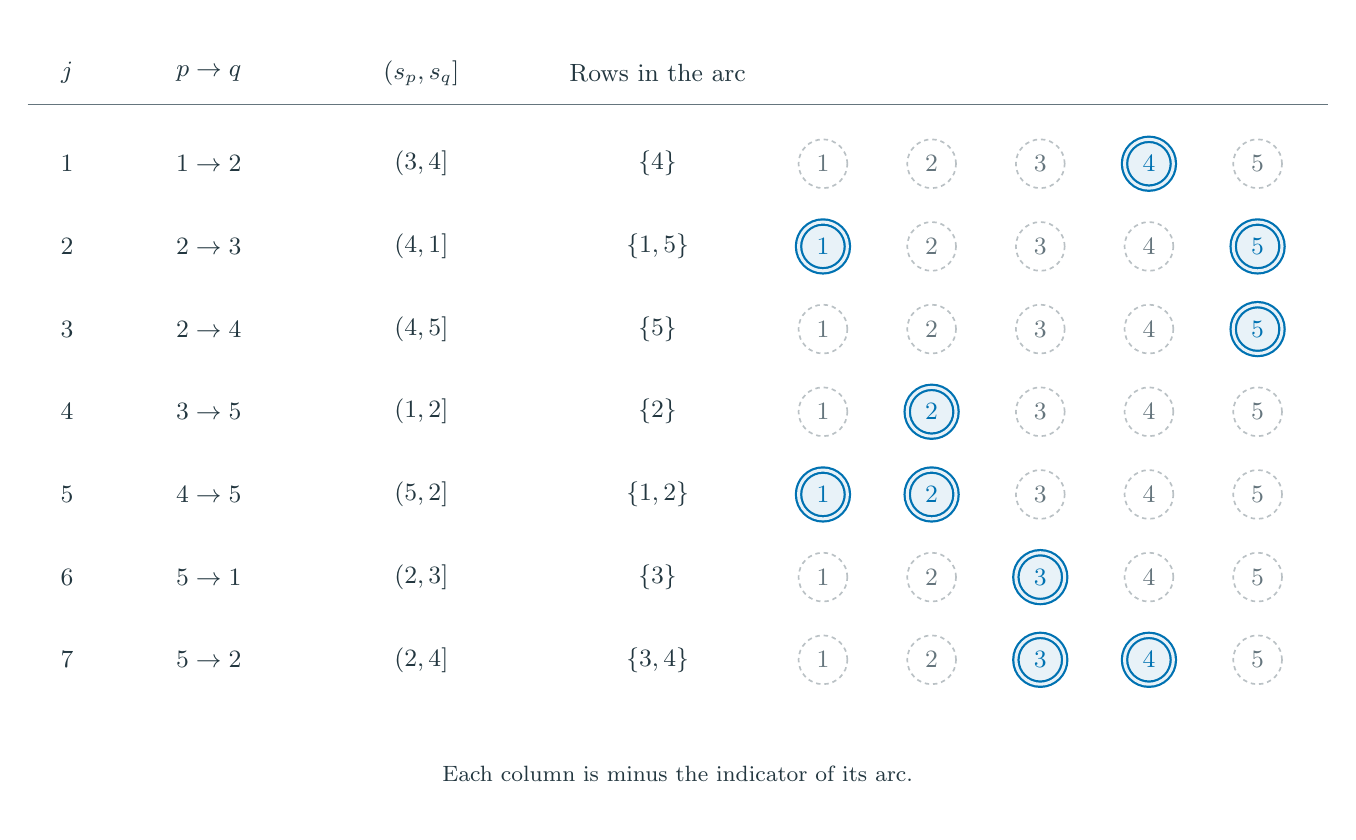
\begin{tikzpicture}[x=1cm,y=1cm]
\useasboundingbox (-0.25000,-9.47802) rectangle (16.26000,0.47802);
\node[ttl] at (0.250,-0.100) {$j$}; %t j
\node[ttl] at (2.050,-0.100) {$p\to q$}; %t edge
\node[ttl] at (4.750,-0.100) {$(s_{p},s_{q}]$}; %t arc
\node[ttl] at (7.750,-0.100) {Rows in the arc}; %t rows
\draw[base] (-0.250,-0.5) -- (16.260,-0.5);
\node[labm] at (0.250,-1.250) {$1$}; %t j0
\node[labm] at (2.050,-1.250) {$1\to 2$}; %t edge0
\node[labm] at (4.750,-1.250) {$(3,4]$}; %t arc0
\node[labm] at (7.750,-1.250) {$\{4\}$}; %t rows0
\node[cellout] at (9.850,-1.250) {1}; %m 1 1 0
\node[cellout] at (11.230,-1.250) {2}; %m 1 2 0
\node[cellout] at (12.610,-1.250) {3}; %m 1 3 0
\node[cellin] at (13.990,-1.250) {4}; %m 1 4 1
\node[cellout] at (15.370,-1.250) {5}; %m 1 5 0
\node[labm] at (0.250,-2.300) {$2$}; %t j1
\node[labm] at (2.050,-2.300) {$2\to 3$}; %t edge1
\node[labm] at (4.750,-2.300) {$(4,1]$}; %t arc1
\node[labm] at (7.750,-2.300) {$\{1,5\}$}; %t rows1
\node[cellin] at (9.850,-2.300) {1}; %m 2 1 1
\node[cellout] at (11.230,-2.300) {2}; %m 2 2 0
\node[cellout] at (12.610,-2.300) {3}; %m 2 3 0
\node[cellout] at (13.990,-2.300) {4}; %m 2 4 0
\node[cellin] at (15.370,-2.300) {5}; %m 2 5 1
\node[labm] at (0.250,-3.350) {$3$}; %t j2
\node[labm] at (2.050,-3.350) {$2\to 4$}; %t edge2
\node[labm] at (4.750,-3.350) {$(4,5]$}; %t arc2
\node[labm] at (7.750,-3.350) {$\{5\}$}; %t rows2
\node[cellout] at (9.850,-3.350) {1}; %m 3 1 0
\node[cellout] at (11.230,-3.350) {2}; %m 3 2 0
\node[cellout] at (12.610,-3.350) {3}; %m 3 3 0
\node[cellout] at (13.990,-3.350) {4}; %m 3 4 0
\node[cellin] at (15.370,-3.350) {5}; %m 3 5 1
\node[labm] at (0.250,-4.400) {$4$}; %t j3
\node[labm] at (2.050,-4.400) {$3\to 5$}; %t edge3
\node[labm] at (4.750,-4.400) {$(1,2]$}; %t arc3
\node[labm] at (7.750,-4.400) {$\{2\}$}; %t rows3
\node[cellout] at (9.850,-4.400) {1}; %m 4 1 0
\node[cellin] at (11.230,-4.400) {2}; %m 4 2 1
\node[cellout] at (12.610,-4.400) {3}; %m 4 3 0
\node[cellout] at (13.990,-4.400) {4}; %m 4 4 0
\node[cellout] at (15.370,-4.400) {5}; %m 4 5 0
\node[labm] at (0.250,-5.450) {$5$}; %t j4
\node[labm] at (2.050,-5.450) {$4\to 5$}; %t edge4
\node[labm] at (4.750,-5.450) {$(5,2]$}; %t arc4
\node[labm] at (7.750,-5.450) {$\{1,2\}$}; %t rows4
\node[cellin] at (9.850,-5.450) {1}; %m 5 1 1
\node[cellin] at (11.230,-5.450) {2}; %m 5 2 1
\node[cellout] at (12.610,-5.450) {3}; %m 5 3 0
\node[cellout] at (13.990,-5.450) {4}; %m 5 4 0
\node[cellout] at (15.370,-5.450) {5}; %m 5 5 0
\node[labm] at (0.250,-6.500) {$6$}; %t j5
\node[labm] at (2.050,-6.500) {$5\to 1$}; %t edge5
\node[labm] at (4.750,-6.500) {$(2,3]$}; %t arc5
\node[labm] at (7.750,-6.500) {$\{3\}$}; %t rows5
\node[cellout] at (9.850,-6.500) {1}; %m 6 1 0
\node[cellout] at (11.230,-6.500) {2}; %m 6 2 0
\node[cellin] at (12.610,-6.500) {3}; %m 6 3 1
\node[cellout] at (13.990,-6.500) {4}; %m 6 4 0
\node[cellout] at (15.370,-6.500) {5}; %m 6 5 0
\node[labm] at (0.250,-7.550) {$7$}; %t j6
\node[labm] at (2.050,-7.550) {$5\to 2$}; %t edge6
\node[labm] at (4.750,-7.550) {$(2,4]$}; %t arc6
\node[labm] at (7.750,-7.550) {$\{3,4\}$}; %t rows6
\node[cellout] at (9.850,-7.550) {1}; %m 7 1 0
\node[cellout] at (11.230,-7.550) {2}; %m 7 2 0
\node[cellin] at (12.610,-7.550) {3}; %m 7 3 1
\node[cellin] at (13.990,-7.550) {4}; %m 7 4 1
\node[cellout] at (15.370,-7.550) {5}; %m 7 5 0
\node[lab] at (8.005,-9.000) {Each column is minus the indicator of its arc.}; %t reading
\end{tikzpicture}
\end{document}
